\documentclass[11pt,a4paper]{report}
\usepackage[textwidth=37em,vmargin=30mm]{geometry}
\usepackage{calc,xunicode,amsmath,amssymb,paralist,enumitem,tabu,booktabs,datetime2,xeCJK,xeCJKfntef,listings}
\usepackage{tocloft,fancyhdr,tcolorbox,xcolor,graphicx,eso-pic,xltxtra,xelatexemoji}

\newcommand{\envyear}[0]{2025}
\newcommand{\envdatestr}[0]{2025-04-25}
\newcommand{\envfinaldir}[0]{webdb/2025/20250425/final}

\usepackage[hidelinks]{hyperref}
\hypersetup{
    colorlinks=false,
    pdfpagemode=FullScreen,
    pdftitle={Web Digest - \envdatestr}
}

\setlength{\cftbeforechapskip}{10pt}
\renewcommand{\cftchapfont}{\rmfamily\bfseries\large\raggedright}
\setlength{\cftbeforesecskip}{2pt}
\renewcommand{\cftsecfont}{\sffamily\small\raggedright}

\setdefaultleftmargin{2em}{2em}{1em}{1em}{1em}{1em}

\usepackage{xeCJK,xeCJKfntef}
\xeCJKsetup{PunctStyle=plain,RubberPunctSkip=false,CJKglue=\strut\hskip 0pt plus 0.1em minus 0.05em,CJKecglue=\strut\hskip 0.22em plus 0.2em}
\XeTeXlinebreaklocale "zh"
\XeTeXlinebreakskip = 0pt


\setmainfont{Brygada 1918}
\setromanfont{Brygada 1918}
\setsansfont{IBM Plex Sans}
\setmonofont{JetBrains Mono NL}
\setCJKmainfont{Noto Serif CJK SC}
\setCJKromanfont{Noto Serif CJK SC}
\setCJKsansfont{Noto Sans CJK SC}
\setCJKmonofont{Noto Sans CJK SC}

\setlength{\parindent}{0pt}
\setlength{\parskip}{8pt}
\linespread{1.15}

\lstset{
	basicstyle=\ttfamily\footnotesize,
	numbersep=5pt,
	backgroundcolor=\color{black!5},
	showspaces=false,
	showstringspaces=false,
	showtabs=false,
	tabsize=2,
	captionpos=b,
	breaklines=true,
	breakatwhitespace=true,
	breakautoindent=true,
	linewidth=\textwidth
}






\newcommand{\coverpic}[2]{
    % argv: itemurl, authorname
    Cover photo by #2~~(\href{#1}{#1})
}
\newcommand{\makeheader}[0]{
    \begin{titlepage}
        % \newgeometry{hmargin=15mm,tmargin=21mm,bmargin=12mm}
        \begin{center}
            
            \rmfamily\scshape
            \fontspec{BaskervilleF}
            \fontspec{Old Standard}
            \fontsize{59pt}{70pt}\selectfont
            WEB\hfill DIGEST
            
            \vfill
            % \vskip 30pt
            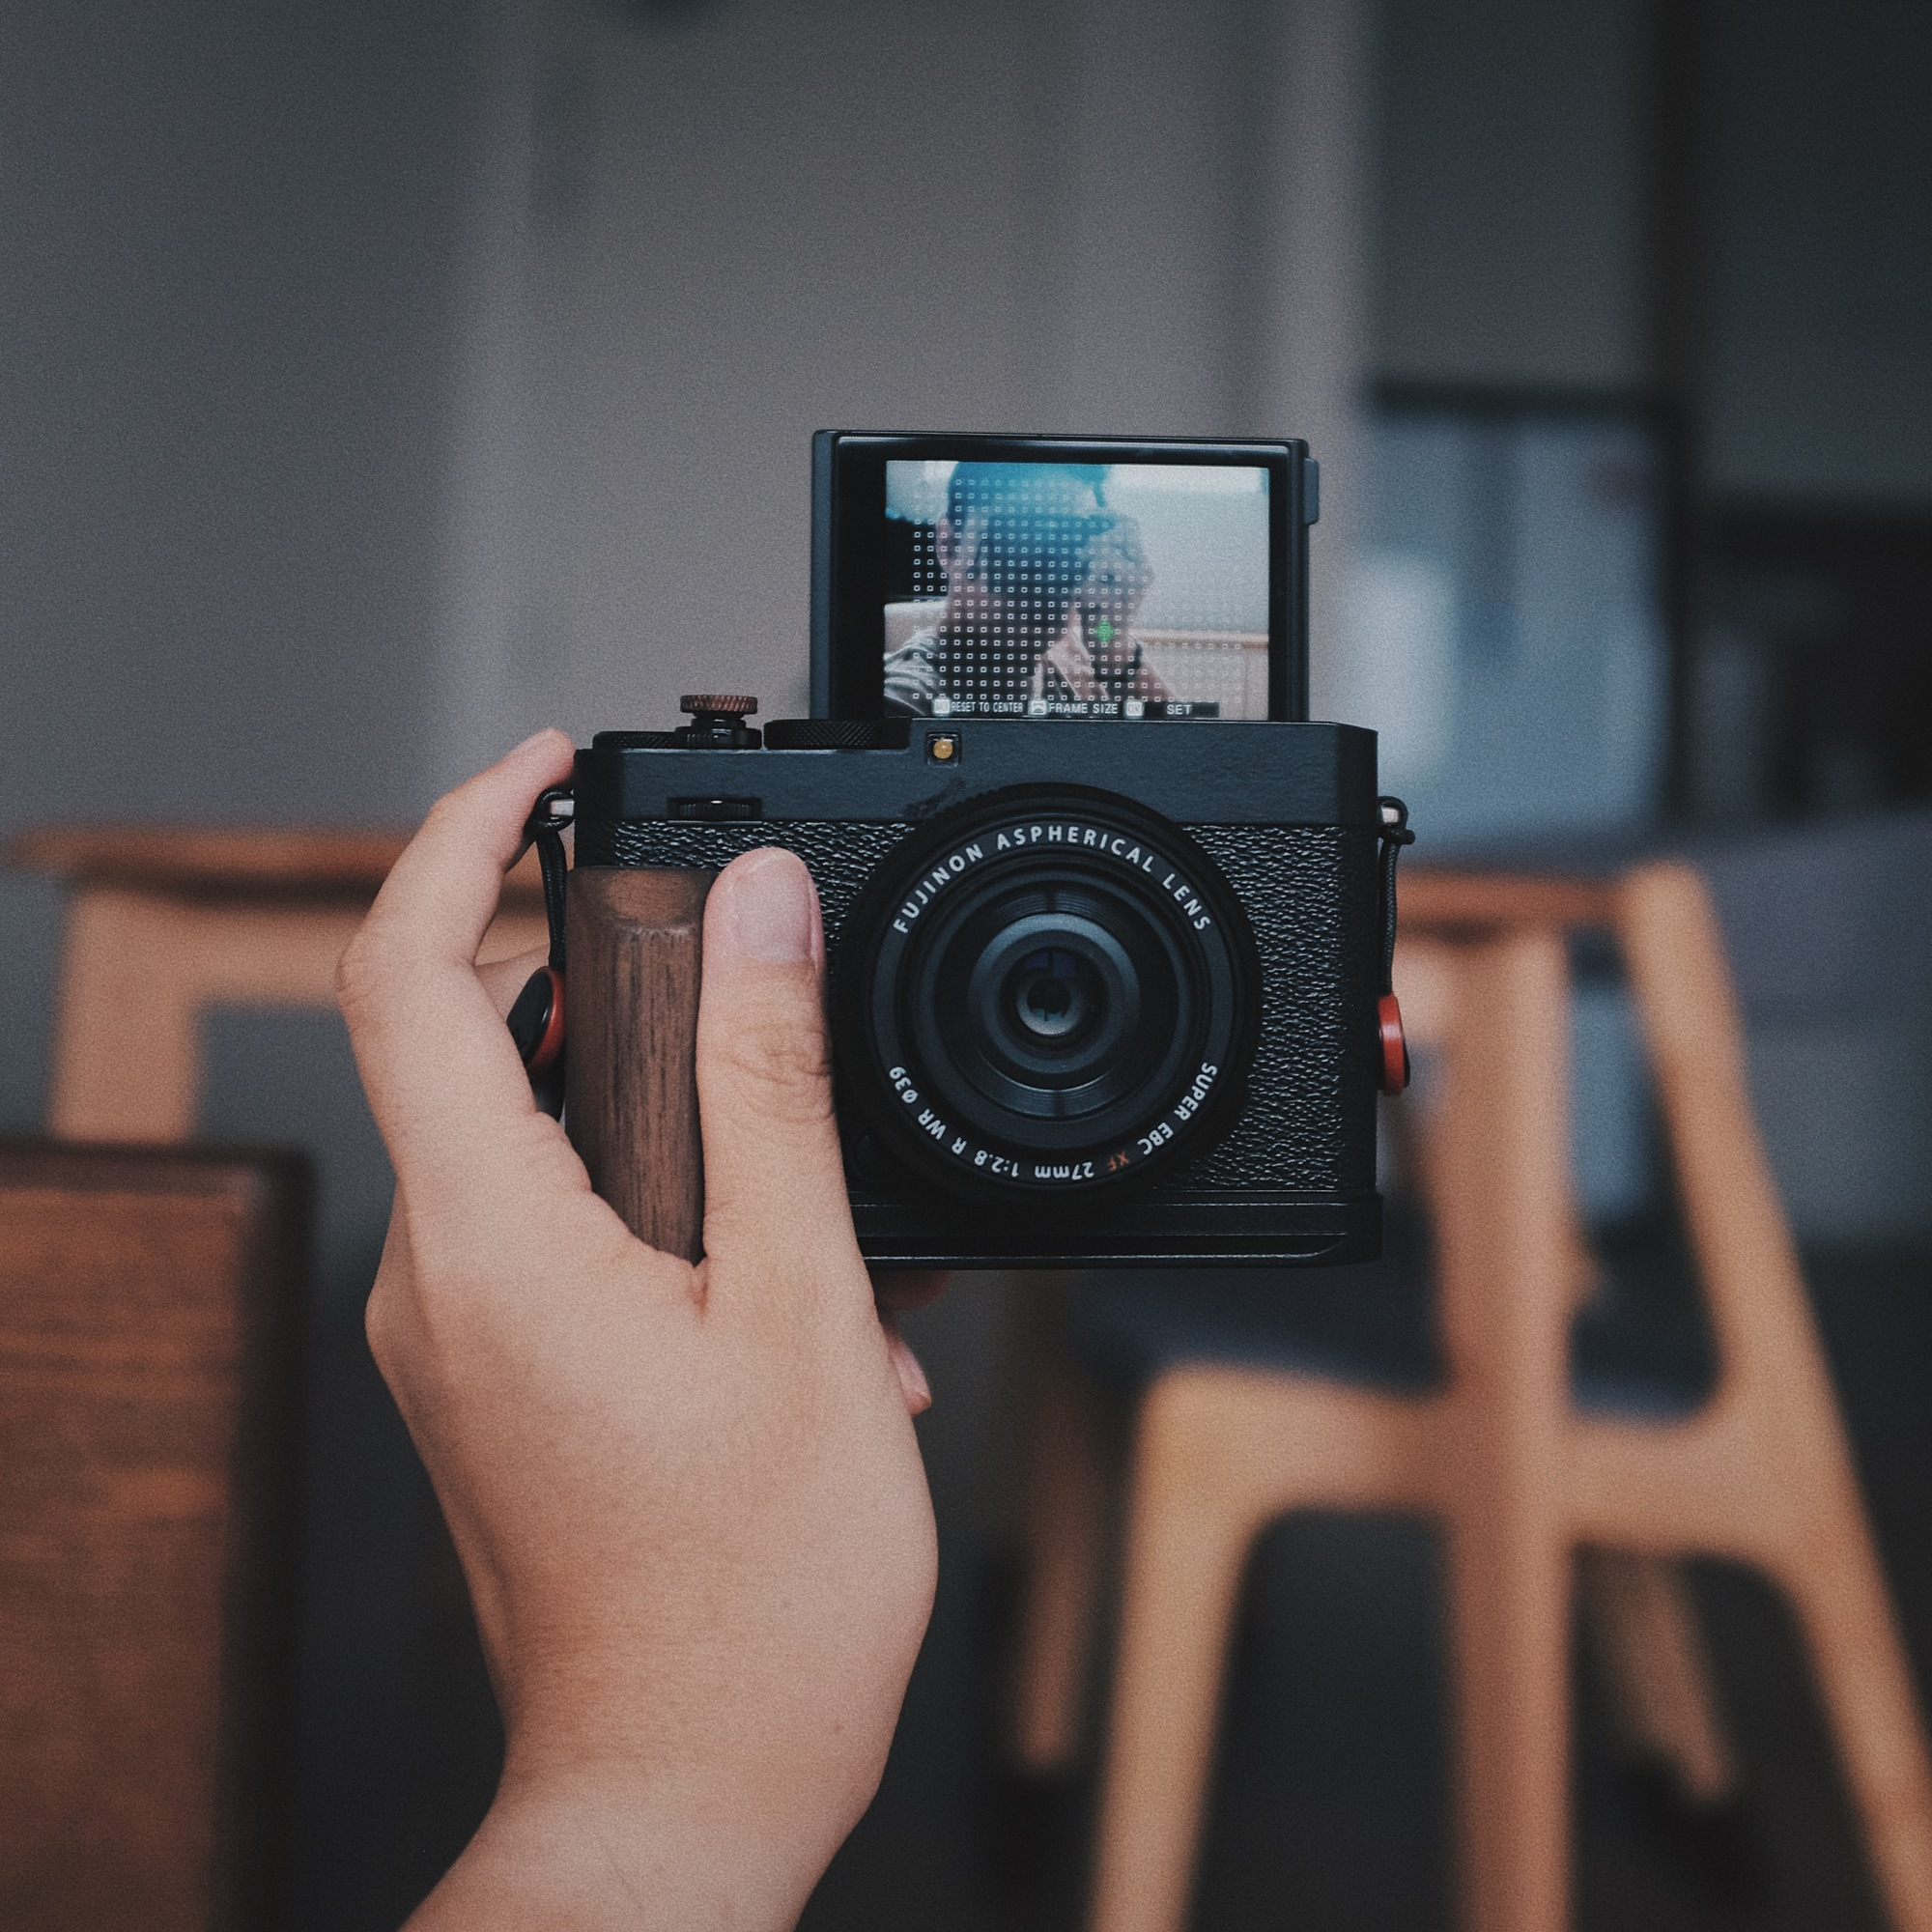
\includegraphics[width=\linewidth]{\envfinaldir/coverpic-prod.jpg}\par
            % \vskip 30pt
            \vfill

            \normalsize\rmfamily\scshape
            \copyright{} The Web Digest Project \hfill\large \envdatestr
        \end{center}
    \end{titlepage}
    % \restoregeometry
}
\newcommand{\simplehref}[1]{%
    \textcolor{blue!80!green}{\href{#1}{#1}}%
}
\renewcommand{\contentsname}{\center\Huge\sffamily\bfseries Contents\par\vskip 20pt}
\newcounter{ipartcounter}
\setcounter{ipartcounter}{0}
\newcommand{\ipart}[1]{
    % \vskip 20pt
    \clearpage
    \stepcounter{ipartcounter}
    \phantomsection
    \addcontentsline{toc}{chapter}{#1}
    % \begin{center}
    %     \Huge
    %     \sffamily\bfseries
    %     #1
    % \end{center}
    % \vskip 20pt plus 7pt
}
\newcounter{ichaptercounter}
\setcounter{ichaptercounter}{0}
\newcommand{\ichapter}[1]{
    % \vskip 20pt
    \clearpage
    \stepcounter{ichaptercounter}
    \phantomsection
    \addcontentsline{toc}{section}{\numberline{\arabic{ichaptercounter}}#1}
    \begin{center}
        \Huge
        \sffamily\bfseries
        #1
    \end{center}
    \vskip 20pt plus 7pt
}
\newcommand{\entrytitlefont}[1]{\subsection*{\raggedright\Large\sffamily\bfseries#1}}
\newcommand{\entryitemGeneric}[2]{
    % argv: title, url
    \parbox{\linewidth}{
        \entrytitlefont{#1}\par\vskip 5pt
        \footnotesize\ttfamily\mdseries
        \simplehref{#2}
    }\vskip 11pt plus 11pt minus 1pt
}
\newcommand{\entryitemGithub}[3]{
    % argv: title, url, desc
    \parbox{\linewidth}{
        \entrytitlefont{#1}\par\vskip 5pt
        \footnotesize\ttfamily\mdseries
        \simplehref{#2}\par\vskip 5pt
        \small\rmfamily\mdseries#3
    }\vskip 11pt plus 11pt minus 1pt
}
\newcommand{\entryitemAp}[3]{
    % argv: title, url, desc
    \parbox{\linewidth}{
        \entrytitlefont{#1}\par\vskip 5pt
        \footnotesize\ttfamily\mdseries
        \simplehref{#2}\par\vskip 5pt
        \small\rmfamily\mdseries#3
    }\vskip 11pt plus 11pt minus 1pt
}
\newcommand{\entryitemHackernews}[3]{
    % argv: title, hnurl, rawurl
    % \parbox{\linewidth}{
    %     \entrytitlefont{#1}\par\vskip 5pt
    %     \footnotesize\ttfamily\mdseries
    %     \simplehref{#3}\par
    %     \textcolor{black!50}{\href{#2}{#2}}
    % }\vskip 11pt plus 11pt minus 1pt
    \begin{minipage}{\linewidth}
            \entrytitlefont{#1}\par\vskip 5pt
            \footnotesize\ttfamily\mdseries
            \simplehref{#3}\par
            \textcolor{black!50}{\href{#2}{#2}}
    \end{minipage}\par\vskip 11pt plus 11pt minus 1pt
}







\begin{document}

\makeheader

\tableofcontents\clearpage




\ipart{Developers}
\ichapter{Hacker News}
\entryitemTwoLinks{OpenAI releases image generation in the API}{https://news.ycombinator.com/item?id=43786506}{https://openai.com/index/image-generation-api/}

\entryitemTwoLinks{NSF director to resign amid grant terminations, job cuts, and controversy}{https://news.ycombinator.com/item?id=43786304}{https://www.science.org/content/article/nsf-director-resign-amid-grant-terminations-job-cuts-and-controversy}

\entryitemTwoLinks{OpenVSX, which VSCode forks rely on for extensions, down for 24 hours}{https://news.ycombinator.com/item?id=43785039}{https://status.open-vsx.org/}

\entryitemTwoLinks{Manufactured consensus on x.com}{https://news.ycombinator.com/item?id=43784915}{https://rook2root.co/articles/20250424-manufacturing-consensus-on-x}

\entryitemTwoLinks{One quantum transition makes light at 21 cm}{https://news.ycombinator.com/item?id=43784721}{https://bigthink.com/starts-with-a-bang/21cm-magic-length/}

\entryitemTwoLinks{Instant SQL for results as you type in DuckDB UI}{https://news.ycombinator.com/item?id=43782406}{https://motherduck.com/blog/introducing-instant-sql/}

\entryitemTwoLinks{Ask HN: Share your AI prompt that stumps every model}{https://news.ycombinator.com/item?id=43782299}{https://news.ycombinator.com/item?id=43782299}

\entryitemTwoLinks{America's reputation drops across the world}{https://news.ycombinator.com/item?id=43782159}{https://www.ipsos.com/en/americas-reputation-drops-across-the-world}

\entryitemTwoLinks{I wrote to the address in the GPLv2 license notice (2022)}{https://news.ycombinator.com/item?id=43781888}{https://code.mendhak.com/gpl-v2-address-letter/}

\entryitemTwoLinks{Assignment 5: Cars and Key Fobs}{https://news.ycombinator.com/item?id=43780876}{https://web.stanford.edu/class/ee26n/Assignments/Assignment5.html}

\entryitemTwoLinks{On loyalty to your employer (2018)}{https://news.ycombinator.com/item?id=43780815}{https://medium.com/hackernoon/on-loyalty-to-your-employer-c674c4b06b3a}

\entryitemTwoLinks{Creating your own federated microblog}{https://news.ycombinator.com/item?id=43780785}{https://fedify.dev/tutorial/microblog}

\entryitemTwoLinks{Vim Language, Motions, and Modes Explained (2023)}{https://news.ycombinator.com/item?id=43780682}{https://www.ssp.sh/blog/why-using-neovim-data-engineer-and-writer-2023/}

\entryitemTwoLinks{Mark Zuckerberg says social media is over}{https://news.ycombinator.com/item?id=43780377}{https://www.newyorker.com/culture/infinite-scroll/mark-zuckerberg-says-social-media-is-over}

\entryitemTwoLinks{Careless People}{https://news.ycombinator.com/item?id=43780363}{https://pluralistic.net/2025/04/23/zuckerstreisand/\#zdgaf}

\entryitemTwoLinks{AMD Publishes Open-Source Driver for GPU Virtualization, Radeon "In the Roadmap"}{https://news.ycombinator.com/item?id=43779953}{https://www.phoronix.com/news/AMD-GIM-Open-Source}

\entryitemTwoLinks{Daily driving a Linux phone, but why?}{https://news.ycombinator.com/item?id=43779766}{https://thefoggiest.dev/2025/04/24/daily-driving-a-linux-phone-but-why}

\entryitemTwoLinks{Shortest-possible walking tour to 81,998 bars in South Korea}{https://news.ycombinator.com/item?id=43778105}{https://www.math.uwaterloo.ca/tsp/korea/index.html}

\entryitemTwoLinks{Show HN: My from-scratch OS kernel that runs DOOM}{https://news.ycombinator.com/item?id=43778081}{https://github.com/UnmappedStack/TacOS}

\entryitemTwoLinks{CubeCL: GPU Kernels in Rust for CUDA, ROCm, and WGPU}{https://news.ycombinator.com/item?id=43777731}{https://github.com/tracel-ai/cubecl}\ichapter{Phoronix}
\entryitemGeneric{\hskip 0pt{}Lenovo ThinkPad X1 Carbon Gen 13 Aura Can Work Well As A Solid Linux Laptop}{https://www.phoronix.com/review/lenovo-thinkpad-x1-gen13-linux}

\entryitemGeneric{\hskip 0pt{}SCALE 1.3 Adds BFloat16 \& Other New Features For Compiling CUDA Apps On AMD GPUs}{https://www.phoronix.com/news/SCALE-1.3-Released}

\entryitemGeneric{\hskip 0pt{}Linux 6.15 Fixes A Performance Issue For Extremely Heavy Read-Only Workloads}{https://www.phoronix.com/news/Linux-6.15-Extreme-Heavy-Reads}

\entryitemGeneric{\hskip 0pt{}New Patches Get Linux Booting On The Snapdragon X1-Powered Dell Inspiron 14 Plus}{https://www.phoronix.com/news/Dell-Inspiron-14-Plus-Linux-X1E}

\entryitemGeneric{\hskip 0pt{}Mesa Falling Back To Its Multi-File Cache Due To Performance Reasons}{https://www.phoronix.com/news/Mesa-Single-File-Cache-Issue}

\entryitemGeneric{\hskip 0pt{}Raspberry Pi HEVC Decoder Linux Driver Updated For Mainline Kernel Attempt}{https://www.phoronix.com/news/Raspberry-Pi-HEVC-Decode-V3}

\entryitemGeneric{\hskip 0pt{}PCIe Controller Support For The Apple M2 Pro Coming To The Mainline Linux Kernel}{https://www.phoronix.com/news/Apple-T6020-PCIe-M2-Pro}

\entryitemGeneric{\hskip 0pt{}AMD Publishes Open-Source GIM Driver For GPU Virtualization, Radeon "In The Roadmap"}{https://www.phoronix.com/news/AMD-GIM-Open-Source}

\entryitemGeneric{\hskip 0pt{}OpenMandriva Lx 6.0 Brings KDE Plasma 6 By Default, Official Server Edition}{https://www.phoronix.com/news/OpenMandriva-Lx-6.0-Released}\ichapter{GitHub}
\entryitemWithDescription{\hskip 0pt{}khoj-ai/khoj}{https://github.com/khoj-ai/khoj}{Your AI second brain. Self-hostable. Get answers from the web or your
docs. Build custom agents, schedule automations, do deep research. Turn
any online or local LLM into your personal, autonomous AI (gpt, claude,
gemini, llama, qwen, mistral). Get started - free.\\
Language: Python\\
Stars: 28983\\
Forks: 1618}\ichapter{Dribbble}
\entryitemGeneric{\hskip 0pt{}Bismuth}{https://dribbble.com/shots/25942596-Bismuth}

\entryitemGeneric{\hskip 0pt{}Betpanda}{https://dribbble.com/shots/25937317-Betpanda}

\entryitemGeneric{\hskip 0pt{}Travel Startup Branding for Holidu: visual identity brand design}{https://dribbble.com/shots/25916676-Travel-Startup-Branding-for-Holidu-visual-identity-brand-design}

\entryitemGeneric{\hskip 0pt{}Unused Netomi Logo Concept}{https://dribbble.com/shots/25937558-Unused-Netomi-Logo-Concept}

\entryitemGeneric{\hskip 0pt{}Crypto Portfolio Tracker App}{https://dribbble.com/shots/25936470-Crypto-Portfolio-Tracker-App}

\entryitemGeneric{\hskip 0pt{}Geometric M Logo Design - Letter, Monogram}{https://dribbble.com/shots/25936398-Geometric-M-Logo-Design-Letter-Monogram}

\entryitemGeneric{\hskip 0pt{}RedBird Films}{https://dribbble.com/shots/25938378-RedBird-Films}

\entryitemGeneric{\hskip 0pt{}Hand-Lettering Samples v1}{https://dribbble.com/shots/25938484-Hand-Lettering-Samples-v1}

\entryitemGeneric{\hskip 0pt{}Colorful M - Logo Design // For SALE}{https://dribbble.com/shots/25937554-Colorful-M-Logo-Design-For-SALE}

\entryitemGeneric{\hskip 0pt{}Fundly Branding - Fintech company}{https://dribbble.com/shots/25936018-Fundly-Branding-Fintech-company}

\entryitemGeneric{\hskip 0pt{}Bismuth}{https://dribbble.com/shots/25933886-Bismuth}

\entryitemGeneric{\hskip 0pt{}boundless}{https://dribbble.com/shots/25930426-boundless}

\entryitemGeneric{\hskip 0pt{}Logo Design for Premium Online Store}{https://dribbble.com/shots/25931384-Logo-Design-for-Premium-Online-Store}

\entryitemGeneric{\hskip 0pt{}Answering Agent AI}{https://dribbble.com/shots/25932675-Answering-Agent-AI}

\entryitemGeneric{\hskip 0pt{}Visual Identity: Biometric verification layer for secure Web3}{https://dribbble.com/shots/25931676-Visual-Identity-Biometric-verification-layer-for-secure-Web3}

\entryitemGeneric{\hskip 0pt{}Tempora Logo Design - Hourglass, Time, Sand Clock}{https://dribbble.com/shots/25926528-Tempora-Logo-Design-Hourglass-Time-Sand-Clock}

\entryitemGeneric{\hskip 0pt{}OltreFluire}{https://dribbble.com/shots/25914855-OltreFluire}

\entryitemGeneric{\hskip 0pt{}Website for a Fintech Company ✦ Kony}{https://dribbble.com/shots/25927385-Website-for-a-Fintech-Company-Kony}

\entryitemGeneric{\hskip 0pt{}Cruising for the coast}{https://dribbble.com/shots/25914452-Cruising-for-the-coast}

\entryitemGeneric{\hskip 0pt{}Tanuki - Raccoon, Animal Logo Design}{https://dribbble.com/shots/25917338-Tanuki-Raccoon-Animal-Logo-Design}

\entryitemGeneric{\hskip 0pt{}Bismuth}{https://dribbble.com/shots/25918310-Bismuth}

\entryitemGeneric{\hskip 0pt{}Logo Design for AI Companies}{https://dribbble.com/shots/25917078-Logo-Design-for-AI-Companies}

\entryitemGeneric{\hskip 0pt{}American Home Shield}{https://dribbble.com/shots/25916194-American-Home-Shield}

\entryitemGeneric{\hskip 0pt{}Blockio responsive}{https://dribbble.com/shots/25915933-Blockio-responsive}


\ipart{Developers~~~~(zh-Hans)}
\ichapter{Solidot}
\entryitemGeneric{\hskip 0pt{}神舟二十号成功发射}{https://www.solidot.org/story?sid=81143}

\entryitemGeneric{\hskip 0pt{}哈勃在轨运行 35 周年}{https://www.solidot.org/story?sid=81142}

\entryitemGeneric{\hskip 0pt{}随着研究资金缩减更多美国科学家前往海外}{https://www.solidot.org/story?sid=81141}

\entryitemGeneric{\hskip 0pt{}21 世纪至今引用次数最高的论文}{https://www.solidot.org/story?sid=81140}

\entryitemGeneric{\hskip 0pt{}用户使用 AI 的需求发生了改变}{https://www.solidot.org/story?sid=81139}

\entryitemGeneric{\hskip 0pt{}科学家称发现一种全新的颜色}{https://www.solidot.org/story?sid=81138}

\entryitemGeneric{\hskip 0pt{}研究人员证明走遍韩国 8 万酒吧的最短路径}{https://www.solidot.org/story?sid=81137}

\entryitemGeneric{\hskip 0pt{}Google Gemini 有 3.5 亿月活用户}{https://www.solidot.org/story?sid=81136}

\entryitemGeneric{\hskip 0pt{}Discord 准备 IPO,CEO 兼联合创始人辞职}{https://www.solidot.org/story?sid=81135}

\entryitemGeneric{\hskip 0pt{}Google 强迫部分远程工作员工回办公室工作否则面临解雇}{https://www.solidot.org/story?sid=81134}

\entryitemGeneric{\hskip 0pt{}亚洲的 IPv6 覆盖率超过五成}{https://www.solidot.org/story?sid=81133}

\entryitemGeneric{\hskip 0pt{}世界模型真要来了?Google 的第三代Dreamer算法,除了能完成150余种不同控制任务,还能在《我的世界》里找到钻石}{https://www.solidot.org/story?sid=81132}

\entryitemGeneric{\hskip 0pt{}YouTube 用户上传了 20 万亿则视频}{https://www.solidot.org/story?sid=81130}

\entryitemGeneric{\hskip 0pt{}苹果和 Meta 因违反欧盟《数字市场法》分别被罚 5 亿和 2 亿欧元}{https://www.solidot.org/story?sid=81129}

\entryitemGeneric{\hskip 0pt{}QEMU 10.0 释出}{https://www.solidot.org/story?sid=81128}

\entryitemGeneric{\hskip 0pt{}昆虫在全世界以惊人的速度消失}{https://www.solidot.org/story?sid=81127}

\entryitemGeneric{\hskip 0pt{}脉冲星揭示星际等离子体结构}{https://www.solidot.org/story?sid=81126}

\entryitemGeneric{\hskip 0pt{}Google Chrome 将继续使用第三方 Cookies }{https://www.solidot.org/story?sid=81125}

\entryitemGeneric{\hskip 0pt{}英特尔计划裁掉逾五分之一员工}{https://www.solidot.org/story?sid=81124}

\entryitemGeneric{\hskip 0pt{}OpenAI 有意收购 Chrome}{https://www.solidot.org/story?sid=81123}\ichapter{V2EX}
\entryitemGeneric{\hskip 0pt{}[分享发现] 现在的学生更可怜了}{https://www.v2ex.com/t/1127918}

\entryitemGeneric{\hskip 0pt{}[YouTube] YouTube 后台播放不能关?}{https://www.v2ex.com/t/1127917}

\entryitemGeneric{\hskip 0pt{}[问与答] windows 上,有没有图片查看软件推荐?}{https://www.v2ex.com/t/1127915}

\entryitemGeneric{\hskip 0pt{}[推广] 铅基超导体研发突破, ROOMCON 去中心化科研体系取得新进展}{https://www.v2ex.com/t/1127914}

\entryitemGeneric{\hskip 0pt{}[程序员] 关于 gin+xhtml 和 next nuxt 的对比,各位兄弟们看看}{https://www.v2ex.com/t/1127913}

\entryitemGeneric{\hskip 0pt{}[宽带症候群] 重庆联通现在也开始回收公网动态 IP 了?我才发现拨出来的全是内网 IP 段}{https://www.v2ex.com/t/1127912}

\entryitemGeneric{\hskip 0pt{}[JetBrains] jb 这个定价策略是不是有点过于歧视国区了?}{https://www.v2ex.com/t/1127911}

\entryitemGeneric{\hskip 0pt{}[分享创造] 分享一个体感手势控制的虚拟手枪 iOS / iWatch App,用 Swift 写的}{https://www.v2ex.com/t/1127910}

\entryitemGeneric{\hskip 0pt{}[分享发现] 喜欢玩射击类游戏的宝子,可以试试这两款游戏哇。}{https://www.v2ex.com/t/1127909}

\entryitemGeneric{\hskip 0pt{}[问与答] 很好奇笔记本的官方软件是如何实现控制充电阈值的}{https://www.v2ex.com/t/1127908}

\entryitemGeneric{\hskip 0pt{}[问与答] 请教一下,如何可以用 gmail 注册 Line 的 app 软件?}{https://www.v2ex.com/t/1127906}

\entryitemGeneric{\hskip 0pt{}[NAS] NAS 上部署音乐服务器}{https://www.v2ex.com/t/1127905}

\entryitemGeneric{\hskip 0pt{}[酷工作] [郑州][金融机构][国企]招聘大数据开发工程师、数据架构师、数据开发工程师、算法工程师等}{https://www.v2ex.com/t/1127904}

\entryitemGeneric{\hskip 0pt{}[宽带症候群] 自建 DNS,当域名解析到 CloudFlare 时自动优选 IP}{https://www.v2ex.com/t/1127903}

\entryitemGeneric{\hskip 0pt{}[职场话题] 第一次跳槽,求各位前辈指点}{https://www.v2ex.com/t/1127901}

\entryitemGeneric{\hskip 0pt{}[问与答] steam vr 强制修改电源计划为高性能}{https://www.v2ex.com/t/1127900}

\entryitemGeneric{\hskip 0pt{}[问与答] 求电钢琴推荐}{https://www.v2ex.com/t/1127899}

\entryitemGeneric{\hskip 0pt{}[问与答] 小区住宅晚上 10 点之后还打麻将的人,真的无意识会吵着隔壁左右休息吗?}{https://www.v2ex.com/t/1127898}

\entryitemGeneric{\hskip 0pt{}[酷工作] [合肥] 招聘 AWS 运维工程师 薪资范围 10-15K}{https://www.v2ex.com/t/1127895}

\entryitemGeneric{\hskip 0pt{}[分享创造] 家人们,有鱼摸,速来}{https://www.v2ex.com/t/1127894}

\entryitemGeneric{\hskip 0pt{}[程序员] 35 了 好像没啥特殊感想}{https://www.v2ex.com/t/1127893}

\entryitemGeneric{\hskip 0pt{}[生活] 锅圈食汇有人用过吗?品质怎么样?性价比有吗?}{https://www.v2ex.com/t/1127892}

\entryitemGeneric{\hskip 0pt{}[程序员] AI 进化好快,现在是真能干活}{https://www.v2ex.com/t/1127891}

\entryitemGeneric{\hskip 0pt{}[电影] 动画电影大面积移动镜头时看起来很卡}{https://www.v2ex.com/t/1127890}

\entryitemGeneric{\hskip 0pt{}[macOS] 只用 mac 原生的中文输入法的兄弟来看一下, 在中文输入法下,自动将中文标点替换为英文标点}{https://www.v2ex.com/t/1127889}

\entryitemGeneric{\hskip 0pt{}[问与答] 这几个程序员兼职平台哪个好一些?}{https://www.v2ex.com/t/1127887}

\entryitemGeneric{\hskip 0pt{}[问与答] 请教关于 Windows 桌面开发有关 SendMessage/PostMessaage 的问题.}{https://www.v2ex.com/t/1127886}

\entryitemGeneric{\hskip 0pt{}[程序员] 小红书双休了,咋没看到热帖呢?}{https://www.v2ex.com/t/1127885}

\entryitemGeneric{\hskip 0pt{}[程序员] 性能的终点就是广告吗}{https://www.v2ex.com/t/1127884}

\entryitemGeneric{\hskip 0pt{}[MacBook Pro] M4 macbook pro 15.4.1 今天卡死重启了两次}{https://www.v2ex.com/t/1127882}

\entryitemGeneric{\hskip 0pt{}[问与答] 大伙儿有没有推荐的 filco minila air 键盘 67 配列的键帽 ?}{https://www.v2ex.com/t/1127881}

\entryitemGeneric{\hskip 0pt{}[生活] 简单来说 美团的闪送业务是不是会比京东的本地仓储创建更多区域内就业?}{https://www.v2ex.com/t/1127879}

\entryitemGeneric{\hskip 0pt{}[问与答] 菜鸡求助:如何在 Mac 上设置 Dock 上同一个应用的多个实例的窗口不合并为一个图标?}{https://www.v2ex.com/t/1127878}

\entryitemGeneric{\hskip 0pt{}[iPhone] 4G 和 5G 网络还有假基站么?}{https://www.v2ex.com/t/1127877}

\entryitemGeneric{\hskip 0pt{}[问与答] 京东淘宝可以用一些虚拟卡支付吗}{https://www.v2ex.com/t/1127875}

\entryitemGeneric{\hskip 0pt{}[分享发现] 滴滴企业版似乎总是更快些}{https://www.v2ex.com/t/1127874}

\entryitemGeneric{\hskip 0pt{}[程序员] 使用 v0.dev 写的界面在对话框让他直接对接后端 api 可以吗?}{https://www.v2ex.com/t/1127873}

\entryitemGeneric{\hskip 0pt{}[VPS] 甲骨文大善人也太牛逼了吧}{https://www.v2ex.com/t/1127872}

\entryitemGeneric{\hskip 0pt{}[分享发现] 开源自己用的域名批量扫描工具}{https://www.v2ex.com/t/1127871}

\entryitemGeneric{\hskip 0pt{}[宽带症候群] 坐标南方,最近电信家宽 QoS 严重?}{https://www.v2ex.com/t/1127870}

\entryitemGeneric{\hskip 0pt{}[分享发现] 4-24 黄金收益更新,回血 1600,爽到了,距离回本又进了一步}{https://www.v2ex.com/t/1127869}

\entryitemGeneric{\hskip 0pt{}[随想] 我并不是 AI-proof!}{https://www.v2ex.com/t/1127866}

\entryitemGeneric{\hskip 0pt{}[分享发现] 很奇怪,最近连续做了两个噩梦}{https://www.v2ex.com/t/1127865}

\entryitemGeneric{\hskip 0pt{}[RSS] SeekTab - 重新定义新标签页:内置 RSS 订阅,让信息浏览更高效}{https://www.v2ex.com/t/1127864}

\entryitemGeneric{\hskip 0pt{}[酷工作] 招运维开发工程师 (13-23K)}{https://www.v2ex.com/t/1127863}

\entryitemGeneric{\hskip 0pt{}[问与答] 旧笔记本安装 Proxmox VE(PVE)成功后重启没引导系统怎么回事}{https://www.v2ex.com/t/1127862}

\entryitemGeneric{\hskip 0pt{}[问与答] 据公司内部不可靠消息,公司内部开发了一套俗称牛马系统,老板可以看到每个员工加班时长}{https://www.v2ex.com/t/1127860}

\entryitemGeneric{\hskip 0pt{}[问与答] 怎样处理长期不用的带锂电产品?}{https://www.v2ex.com/t/1127859}

\entryitemGeneric{\hskip 0pt{}[远程工作] 你们都是怎么找远程开发工作的?}{https://www.v2ex.com/t/1127857}

\entryitemGeneric{\hskip 0pt{}[分享发现] 做了个 Memos 客户端欢迎体验}{https://www.v2ex.com/t/1127856}


\ipart{Generic News}
\ichapter{联合早报}
\entryitemWithDescription{韩咏红:特朗普关税从``解放日''走到``妥协日''了?}{https://www.zaobao.com/news/china/story20250425-6240846}{美国总统特朗普在4月2日宣布对等关税政策,短短20天后,特朗普的高姿态已难以为继。特朗普在4月9日就已调整过一次战术,暂缓对其他国家课征对等关税,集中火力单挑中国;而今,特朗普恐怕又要眨眼了,对中国商品课征的145\%关税也可能显著下调。 特朗普近日罕见地对中国伸出橄榄枝,表示考虑大幅度降低对华关税,显露出急于与中国达成协议。但中国偏是表现得不着急……}

\entryitemWithDescription{学者:中国以2+2机制拉拢东南亚国家抗衡美国}{https://www.zaobao.com/news/china/story20250424-6240690}{受访学者分析,在中美关系因贸易战而全面恶化的大背景下,中国正以``外交、国防2+2对话机制''为新抓手,积极拉拢亚细安成员国,以抗衡美国在本区域的影响力,预计中国接下来将推动与更多区域国家建立2+2机制。 中国和印度尼西亚星期一(4月21日)在北京举行外长、防长对话机制下的首次部长级会议,两国在2023年就建立2+2对话机制。中国官方称,这是中国在全球建立的首个部长级2+2机制……}

\entryitemWithDescription{中埃空军首次联训 学者:中国初步具备向中东快速战略投送能力}{https://www.zaobao.com/news/china/story20250424-6240357}{中国空军上周派出多架战斗机、预警机、运输机与空中加油机前往埃及,进行两军首次联训。这是中国空军首次以完整作战体系进行跨洲机动。 受访学者认为,这是中国空军现代化进程的里程碑,有助于发展长途奔袭的技战术;这也标志着中国初步具备向中东进行快速战略投送的能力。 据中国国防部消息,中国与埃及两国空军于4月中旬至5月上旬,在埃及空军基地组织代号为``文明之鹰-2025''的联合训练……}

\entryitemWithDescription{台湾收紧民众申领大陆证照规定 持大陆定居证也将被撤销台湾身份}{https://www.zaobao.com/news/china/story20250424-6239789}{(台北综合讯)台湾再度收紧民众申领中国大陆证照的规定,持有大陆定居证的台湾民众也触犯相关法令,将丧失台湾身份。 综合《旺报》与《联合报》报道,台湾行政院公报显示,陆委会近日对《两岸条例》当中规定发布解释函令称,为确保两岸人员单一身份制度,两岸条例规定台湾人民不得在大陆地区``设有户籍'',或领用大陆地区护照,否则将丧失台湾身份……}

\entryitemWithDescription{神舟二十号成功发射 航天员将开展中国首次涡虫空间再生实验}{https://www.zaobao.com/news/china/story20250424-6239950}{(北京综合讯)中国星期四(4月24日)成功发射神舟二十号载人飞船。三名航天员将在空间站驻留约六个月,并开展中国首次涡虫空间再生实验。 综合新华社、央视新闻和《中国青年报》报道,搭载神舟二十号的长征二号F遥二十运载火箭,星期四下午5时17分在甘肃酒泉卫星发射中心点火发射。约10分钟后,神舟二十号与火箭成功分离,进入预定轨道……}

\entryitemWithDescription{台大罢免升温 朝野对抗加剧}{https://www.zaobao.com/news/china/story20250424-6240062}{台湾两大在野党将携手举办大型造势活动,抗议政府利用司法整肃异己,进行大罢免。兼任民进党主席的总统赖清德则公开肯定公民团体罢免在野党立委的行动影片,检调也持续搜索在野国民党宜兰县党部,朝野对抗情势正逐步升温……}

\entryitemWithDescription{美国国会罕见动用传唤权 调查中国三电信巨头}{https://www.zaobao.com/news/china/story20250424-6239456}{(纽约路透电)美国众议院中国问题特别委员会星期三(4月23日)罕见地动用传唤权,调查中国三大电信公司涉嫌支持中国军方和政府的行为。 据路透社报道,中国移动、中国电信和中国联通三家中国电信巨头收到该委员会的传唤通知,须回答他们是否可通过在美开展的云服务和互联网业务获取美国数据的问题。 美国两党议员持续对被指由中国主导的网络攻击事件表示担忧……}

\entryitemWithDescription{浙江一小学门外发生汽车冲撞人群事件}{https://www.zaobao.com/news/china/story20250424-6238514}{(香港综合讯)中国再发生校园伤人事件,浙江金华一所小学门外星期二(4月22日)放学时有汽车冲撞人群,伤亡人数不明。官方在事发两日后仍未发布通报,中国社媒上的相关信息均被删除。 综合《明报》《南华早报》和网媒``香港01''报道,这起事件发生在金华市苏孟乡中心小学门口,时间是星期二傍晚5时45分左右,正值放学时间。附近商户披露,有多名学生被撞……}

\entryitemWithDescription{学者:关税战伤敌一千自损八百 中美终将找到共处之道}{https://www.zaobao.com/news/china/story20250424-6238821}{美国总统特朗普祭出对等关税将届满一个月,如今传出可能降低对华关税,定居美国的资深华人学者赵全胜指出,中美领导阶层有一批人长期相信对方马上要垮台,但关税战让双方意识到,这无疑是``伤敌一千,自损八百'',因此迟早会找到共处之道。 特朗普4月2日宣布全面实施对等关税,随后在9日紧急暂缓90天,让各国争取与美国谈判的时间与空间,唯独对中国不断加码;北京也不甘示弱,提出相应反制……}

\entryitemWithDescription{打击电诈犯罪扩至纵深地带 缅甸向中国移交920余名嫌犯}{https://www.zaobao.com/news/china/story20250424-6238307}{(北京综合讯)中国与缅甸加大打击电信网络诈骗犯罪合作力度,两国最近一个月的合作执法行动,已从缅北地区扩大到当阳、勐休等缅甸纵深地带。 中国公安部官网星期三(4月23日)通报,缅甸执法部门近日将在当地抓获的920余名中国籍涉诈犯罪嫌疑人,通过云南西双版纳打洛口岸全部移交中国警方。 通报称,缅北电诈犯罪集团遭受重创,但部分涉诈人员为逃避打击,向当阳、勐休等纵深地带转移藏匿,继续实施跨境电诈……}

\entryitemWithDescription{沈泽玮:魔幻山城的中国式现代化演绎}{https://www.zaobao.com/news/china/story20250424-6234868}{时隔12年因工作再访重庆,春夏交替之际迎来烈日当空,与当年冬季旅游行走于山城迷雾的印象截然不同。 5000架无人机灯光秀,既展现科技力量也打造视觉盛宴;科企创始人讲述营商环境不断优化;村委会主任手捧涪陵榨菜分享东方酱腌菜``走出去''成果;火车司机传递通关速度如何带动互联互通跨境贸易;公安局交巡警总队科研处综合科科长讲述数字化赋能超大城市治理;社区党委书记分享中国特色``民主村''的前身今世……}

\entryitemWithDescription{中国网购平台将全面取消``仅退款''}{https://www.zaobao.com/news/china/story20250423-6234242}{在中国官方整治``内卷式竞争''的背景下,中国电商平台将全面取消``仅退款''选项。受访学者认为,此举有助行业回归良性竞争,是对电商市场的一次纠偏。 据《北京商报》报道,拼多多、淘宝、抖音、快手、京东等多个中国电商平台,星期二(4月22日)修改有关``仅退款''的相关条款,消费者申请``退款不退货'',将由商家自主处理……}

\entryitemWithDescription{3月人民币跨境收付占比刷新历史纪录}{https://www.zaobao.com/news/china/story20250423-6233857}{(华盛顿彭博电)随着美元的全球吸引力减弱、中美贸易紧张局势上升,3月中国投资者和贸易公司在国际结算中对人民币的使用大幅增加,创下历史纪录。 彭博社基于中国国家外汇管理局星期二(4月22日)公布的数据计算,3月中国大陆境内个人和机构的跨境业务中,人民币使用占比达 54.3\%,总额7249亿美元(9502亿新元)……}

\entryitemWithDescription{中国首次选拔训练外国航天员 巴基斯坦载荷专家有望进中国空间站短期工作}{https://www.zaobao.com/news/china/story20250423-6233118}{(北京综合讯)中国和巴基斯坦正在巴国开展航天员选拔工作,未来几年内将有一名巴基斯坦航天员有机会进入中国空间站执行短期飞行任务。 综合新华社与《中国航天报》消息,中国载人航天工程新闻发言人林西强星期三(23日)宣布,中巴正在巴基斯坦开展航天员的选拔工作,先在巴基斯坦进行初选,然后在中国进行复选和定选,将选拔两名巴基斯坦航天员到中国参加训练……}

\entryitemWithDescription{李家超:上任三年仅休两天假 为港付出``值得''}{https://www.zaobao.com/news/china/story20250423-6234174}{香港特首李家超近日透露,自己上任即将三年,至今只放过两天假,但他认为担任此职是使命,应把所有时间都投入工作,每当看到市民脸上有笑容,他就觉得一切的付出都``值得''。 李家超平日对个人生活极为低调,他星期二(4月22日)接受香港``now''电视台专访时罕有地谈及个人生活,忆述上任至今只试过两天完整休假,一天用来配眼镜,另一天是陪伴家人到医院……}

\entryitemWithDescription{中国多省公布首季GDP:浙江高技术产业增长快 广东低于全国平均水平}{https://www.zaobao.com/news/china/story20250423-6233417}{(杭州/广州综合讯)中国多个省市陆续公布今年一季度经济数据,坐拥``杭州六小龙''等科创企业的浙江地区生产总值(GDP)同比增长6\%,而传统外贸大省广东同比增长4.1\%,低于全国5.4\%的增幅。 浙江省星期一(4月21日)公布一季度GDP为2万2300亿元(人民币,下同,约4000亿新元),同比增长6%,增幅高于浙江年初设定的5.5\%左右的全年增长目标……}

\entryitemWithDescription{赖清德委任前副总统陈建仁 代表台湾出席教宗方济各丧礼}{https://www.zaobao.com/news/china/story20250423-6232538}{(台北综合讯)台湾外交部与梵蒂冈全力交涉,希望促成台湾总统赖清德参加已故教宗方济各的丧礼弥撒。但在双方会商后,改由台湾前副总统陈建仁代表出席。 台湾外交部星期三(4月23日)在官网发表声明称,经过台梵双方讨论,由于陈健仁曾六度晋见教宗方济各,并获教宗亲自颁授教廷宗座科学院院士证章,与教宗关系深厚,决定由陈建仁担任总统特使,代表台湾出席教宗丧礼……}

\entryitemWithDescription{中国限制韩企向美国国防承包商出口含重稀土产品}{https://www.zaobao.com/news/china/story20250423-6232023}{(伦敦 / 首尔综合讯)中国政府告诫韩国企业不要向美国国防承包商出口含有重稀土矿物的产品,违者可能会受其制裁。这项出口管制或将冲击高度依赖出口的韩国经济。 《韩国经济日报》引述当地生产电力变压器的企业消息人士称,目前已有至少两家生产商接获上述通知。其他收到通知的企业包括生产电池、显示器、电动汽车、航空航天和医疗设备的企业,这些产品都都以稀土为关键原料……}

\entryitemWithDescription{中国扩大试点范围 推动服务业开放提速}{https://www.zaobao.com/news/china/story20250423-6228260}{在中美贸易战升级引发全球不安的背景下,中国政府宣布加快推进服务业扩大开放试点,新增九个试点城市与155项试点任务,并突出对接高标准国际经贸规则。 受访学者认为,中国此举履行了继续推动全球化的承诺,有利于树立与美国贸易保护主义不同的形象,参与相关国际规则制定,并吸引更多外资进入其服务业……}

\entryitemWithDescription{台湾蓝白两党将携手上凯道向赖清德发出怒吼}{https://www.zaobao.com/news/china/story20250422-6228009}{台湾在野的国民党(蓝)主席朱立伦与民众党(白)主席黄国昌,星期二(4月22日)举行在野领袖峰会,双方都认为要抑制总统赖清德的专制独裁,但对于如何``倒赖''尚无具体共识。 朱立伦号召群众星期六(4月26日)到总统府前的凯达格兰大道``战独裁'',也邀黄国昌与会。黄国昌当面应允,称将代表民众党参加这场人民的主场,也期盼民众一起站出来向赖清德发出怒吼……}






\clearpage
\leavevmode\vfill
\footnotesize

Copyright \copyright{} 2023-2025 Neruthes and other contributors.

This document is published with CC BY-NC-ND 4.0 license.

The entries listed in this newsletter may be copyrighted by their respective creators.

This newsletter is generated by the Web Digest project.

The newsletters are also delivered via Telegram channel \CJKunderline{\href{https://t.me/webdigestchannel}{https://t.me/webdigestchannel}}.\\
RSS feed is available at \CJKunderline{\href{https://webdigest.pages.dev/rss.xml}{https://webdigest.pages.dev/rss.xml}}.

This newsletter is available in PDF at
\CJKunderline{\href{https://webdigest.pages.dev/}{https://webdigest.pages.dev/}}.

The source code being used to generate this newsletter is available at\\
\CJKunderline{\href{https://github.com/neruthes/webdigest}{https://github.com/neruthes/webdigest}}.

This newsletter is also available in
\CJKunderline{\href{http://webdigest.pages.dev/readhtml/\envyear/WebDigest-20250425.html}{HTML}} and
\CJKunderline{\href{https://github.com/neruthes/webdigest/blob/master/markdown/\envyear/WebDigest-20250425.md}{Markdown}}.


\coverpic{}{}


\end{document}
